\documentclass[a4paper,11pt]{jsarticle}

% 数式
\usepackage{amsmath,amsfonts}
\usepackage{amsthm}
\usepackage{bm}
\usepackage{mathtools}
\usepackage{amssymb}

% 表
\usepackage[utf8]{inputenc}
\usepackage{diagbox} % 斜線付きセルを作成するために必要
\usepackage{booktabs} % 表の罫線を美しくするために必要
\usepackage{hhline} % 水平罫線を制御するために必要

% 画像
\usepackage[dvipdfmx]{graphicx}
\usepackage{ascmac}
\usepackage{physics}
\usepackage{float} % 追加

% 図
\usepackage[dvipdfmx]{graphicx}
\usepackage{tikz} %図を描く
\usetikzlibrary{positioning, intersections, calc, arrows.meta,math} %tikzのlibrary

% ハイパーリンク
\usepackage[dvipdfm,
  colorlinks=false,
  bookmarks=true,
  bookmarksnumbered=false,
  pdfborder={0 0 0},
  bookmarkstype=toc]{hyperref}

% 式番号を章ごとにリセット
\numberwithin{equation}{section}

\begin{document}

\title{非平衡統計力学}
\author{大上由人}
\date{\today}
\maketitle

\tableofcontents
\newpage


\section{はじめに}
\subsection{モチベーション}
ミクロとマクロの中間である系(メゾスコピック系)について考える。このような系においては、環境との相互作用による物理量のゆらぎが無視できなくなる。このような系について、状態が確率的に変動するとしてモデル化し、熱力学との整合性を考える。\\

\subsection{記号}
記号をまとめておく。\\

\subsubsection{時間反転}
時間反転に関する記号をまとめておく。\\
$\bar{\omega}$は時間反転状態を表す。例えば、ある粒子の状態が位相空間上で$(x,p)$であるとき、この時間反転は$(x,-p)$である。\\
また、物理量について、$A^{\dagger}$は逆向きの経路についての物理量である。また、逆向きの経路の確率や遷移レートについても、$P^{\dagger}$や$R^{\dagger}$と表す。\\

\section{必要な数学}
必要な数学をまとめておく。\\

\subsection{確率微分方程式}
\subsubsection{Markov連鎖}
状態も時間も離散的であるような確率過程を考える。このとき、状態間の遷移は以下のように行われる。
\begin{itembox}[l]{\textbf{Def.確率遷移行列}}
  $p^{n-1}$から$p^{n}$への遷移を表す確率遷移行列を、
  \begin{align}
    p^{n}_i = \sum_{j}T_{ij}p^{n-1}_j
  \end{align}
  により定義する。このとき、
  \begin{align}
    T_{ij} &\geq 0 \quad \text{非負性}\\
    \sum_{i}T_{ij} &= 1 \quad \text{規格化}\\
  \end{align}
  である。
\end{itembox}
このとき、規格化がうまくいっていることは以下のように確かめられる。\\
\begin{align}
  \sum_{i}p^{n}_i &= \sum_{i}\sum_{j}T_{ij}p^{n-1}_j\\
  &= \sum_{j}p^{n-1}_j\sum_{i}T_{ij}\\
  &= \sum_{j}p^{n-1}_j\\
  &= 1
\end{align}

\subsubsection{Markov jump過程}
時間は連続だが状態は離散であるようなものを考える。\\
\begin{itembox}[l]{\textbf{Def.遷移レート行列}}
  以下によって遷移レート行列を定義する:
  \begin{align}
    T_{ij} = \begin{cases}
      R_{ij}(n\Delta) \Delta t & \text{if $i \neq j$}\\
      1-\sum_{k}R_{kj}(n\Delta) \Delta t & \text{if $i = j$}
    \end{cases}
  \end{align}
  ただし、
  \begin{align}
    R_{ij}(t) \geq 0 \quad (i \neq j)\\
    \sum_{i}R_{ij} = 0
  \end{align}
  である。
\end{itembox}

\begin{itembox}[l]{\textbf{Thm.マスター方程式}}
  Markov jump過程において、確率分布は以下に従って時間発展する:
  \begin{align}
    \dv{t}p_i(t) = \sum_{j}R_{ij}p_j(t) 
  \end{align}
\end{itembox}
\textbf{Prf.}\\
\begin{align}
  p_i^{n} &= \sum_{j}T_{ij}p_j^{n-1}
\end{align}
のもとで、
\begin{align}
  p_i^n - p_i^{n-1} &= \sum_{j}T_{ij}p_j^{n-1} - p_i^{n-1}\\
  &= \sum_{j(\neq i)}T_{ij}p_j^{n-1} + T_{ii}p_i^{n-1} - p_i^{n-1}\\
  &= \sum_{j(\neq i)}R_{ij}\Delta t p_j^{n-1} + (1-\sum_{k}R_{ki}\Delta t)p_i^{n-1} - p_i^{n-1}\\
  &= -\sum_{k}R_{ki}\Delta t p_i^{n-1} \Delta t + \sum_{j(\neq i)}R_{ij}p_j^{n-1}\Delta t\\
  &= R_{jj}p_j^{n-1}\Delta t + \sum_{j(\neq i)}R_{ij}p_j^{n-1}\Delta t\\
  &= \sum_{j}R_{ij}p_j^{n-1}\Delta t
\end{align}
となる。したがって、
\begin{align}
  \dv{t}p_i(t) = \lim_{\Delta t \to 0}\frac{p_i^n - p_i^{n-1}}{\Delta t} = \sum_{j}R_{ij}p_j(t)
\end{align}
となる。\qed\\

\begin{itembox}[l]{\textbf{Def.escape rate}}
  状態$i$からそれ以外に遷移する遷移率をescape rateという。すなわち、
  \begin{align}
    e_{i,t} = \sum_{j (\neq i)}R_{ij}
  \end{align}
  をescape rateという。
\end{itembox}

\begin{itembox}[l]{\textbf{Req.escape rateの時間反転不変性}}
  escape rateは時間反転に対して不変である。すなわち、
  \begin{align}
    e_{\omega,t} = e_{\bar{\omega},t}^{\dagger}
  \end{align}
  である。
\end{itembox}


\subsubsection{収束定理}
\begin{itembox}[l]{\textbf{Def.既約}}

\end{itembox}

\begin{itembox}[l]{\textbf{Thm.収束定理}}

\end{itembox}





\subsection{経路積分}

\section{熱力学量の定義}
\subsection{エネルギー、熱、仕事}
まずは、熱力学第一法則を構成するエネルギー、熱、仕事についてみていく。\\
エネルギーは通常力学で用いるハミルトニアンで定義される。このとき、エネルギーについて以下の要請をする。\\
\begin{itembox}[l]{\textbf{Req.エネルギーの時間反転不変性}}
  エネルギーは以下を満たす。
  \begin{align}
    E_{\omega} = E_{\bar{\omega}} = E_{\omega}^{\dagger}
  \end{align}

\end{itembox}

\begin{itembox}[l]{\textbf{Def.熱}}
  状態$\omega$から$\omega'$への遷移において、系が熱浴に放出する熱は以下で定義される:
  \begin{align}
    \hat{Q}_{\omega \to \omega'} = E_{\omega} - E_{\omega'} = \frac{1}{\beta}\ln \frac{P_{\omega \to \omega'}}{P_{\omega' \to \omega}^{\dagger}}
  \end{align}
\end{itembox}

\begin{itembox}[l]{\textbf{Def.仕事}}
  系の状態が$\omega$であるとする。このとき、系への仕事は制御パラメータ$\lambda$がポテンシャルを変化させることによって行われる。単位時間あたりに系が外部へ取り出す仕事の量は、以下で定義される:
  \begin{align}
    \hat{\dot{W}} = -\dv{E^{\lambda(t)}_{\omega}}{\lambda(t)}\dv{\lambda(t)}{t}
  \end{align}
\end{itembox}
以上の定義から、熱力学第一法則は以下のように書くことができる:
\begin{align}
  W + Q = -\Delta E
\end{align}
ただし、$\Delta E$は系の平均のエネルギーである。\\

また、系のエントロピーは以下のShanonエントロピーで定義される:

\begin{itembox}[l]{\textbf{Def.エントロピー/自己情報量}}
  系がっかう率分布$\vb{p}$に従うとき、系のShanonエントロピーは以下で定義される:
  \begin{align}
    S(\vb{p}) = -\sum_{\omega}p_{\omega}\ln p_{\omega}
  \end{align}
  また、この量は、$-\log p_{\omega}$の期待値である。このとき、
  \begin{align}
    s(\omega) = -\ln p_{\omega}
  \end{align}
  を自己情報量という。
\end{itembox}


非平衡統計力学において第二法則を考えるときは、エントロピーではなく、以下のエントロピー生成について考える。\\
\begin{itembox}[l]{\textbf{Def.エントロピー生成/エントロピー生成率}}
  時刻$0$から$\tau$の間のエントロピー生成は以下で定義される:
  \begin{align}
    \hat{\sigma} = \sum_{\nu} \beta_{\nu}\hat{Q}_{\nu} + \hat{s}(\omega(\tau)) - \hat{s}(\omega(0))
  \end{align}
  また、  時刻$0$から$\tau$の間の平均のエントロピー生成は以下で定義される:
  \begin{align}
    \sigma &= \expval{\hat{\sigma}}\\
    &= \sum_{\nu} \beta_{\nu} Q_{\nu} + S(\vb{p}(\tau)) - S(\vb{p}(0))
  \end{align}
  また、単位時間当たりのエントロピー生成をエントロピー生成率といい、以下のように書くことができる:
  \begin{align}
    \dot{\sigma} = \sum_{\omega,\omega'}p_{\omega}P_{\omega \to \omega'}\ln \frac{p_{\omega}P_{\omega \to \omega'}}{p_{\omega'}P_{\omega' \to \omega}} \label{eq:EPR}
  \end{align}
\end{itembox}
($\because$(エントロピーの生成率の表式が(\ref{eq:EPR})式であることの証明))\\
この系と熱浴の項はそれぞれ次のように計算される。
この系と熱浴の項はそれぞれ次のように計算される。

\begin{align}
\frac{d}{dt} H(\mathbf{p}(t)) &= - \frac{d}{dt} \sum_w p_w \ln p_w \\
&= - \sum_w \frac{dp_w}{dt} \ln p_w
\end{align}

第2項は確率の規格化から消える。第1項にマスター方程式を代入して

\begin{align}
&= \sum_w \left( \sum_{w'(\neq w), \nu} p_w P_{w \to w'}^\nu - p_{w'} P_{w' \to w}^\nu \right) \ln p_w
\end{align}

和の記号は正確には熱浴の区別 $\omega, \omega'$ 的なものが入るべきであるが,教科書にノーテーションを合わせる。

\begin{align}
&= \sum_{\omega, \omega'} \left( p_{\omega'} P_{\omega' \rightarrow \omega} - p_\omega P_{\omega \rightarrow \omega'} \right) \ln p_\omega \\
&(\text{第2項の添字を入れ替えて})\\
&= \sum_{w, w'} p_w P_{w \to w'} \ln p_w - \sum_{w, w'} p_w P_{w \to w'} \ln p_{w'} \\
&= \sum_{w, w'} p_w P_{w \to w'} \ln \frac{p_w}{p_{w'}}
\end{align}

\begin{align}
\sum_{\nu=1}^{k} \beta_\nu \dot{Q}_\nu &= \sum_{\nu} \beta_\nu \left( \frac{1}{\beta_\nu} \sum_w \frac{dp_w}{dt} \ln \frac{P_{w \to w'}^\nu}{P_{w' \to \overline{w}}^{\dagger, \nu}} \right)\\
&= \sum_{\nu} \sum_{w, w'} p_w P_{w \to w'}^\nu \ln \frac{P_{w \to w'}^\nu}{P_{w' \to \overline{w}}^{\dagger, \nu}}\\
\end{align}
以上より示された。\\
このとき、KLダイバージェンスの非負性から、エントロピー生成率は非負であることがわかる。\\

\subsection{詳細つり合い条件}
非平衡統計力学においては、以下のように平衡状態を定義する。
\begin{itembox}[l]{\textbf{Def.平衡状態}}
  系が平衡状態にあるとは、
  \begin{align}
    p_{\omega}^{\text{eq}}P_{\omega \to \omega'} = p_{\bar{\omega'}}^{\text{eq}}P_{\bar{\omega'} \to \bar{\omega}}^{\dagger}
  \end{align}
  が成り立つことである。

\end{itembox}

また、物理的に有効であるような確率過程においては、以下の条件が成り立つと考えられる。
\begin{itembox}[l]{\textbf{Def.詳細つり合い条件}}
  任意の状態$\omega,\omega'$および定常状態$p^{\text{ss}}_{\omega},p^{\text{ss}}_{\omega'}$に対して、以下の条件が成り立つとき、系は詳細つり合い条件を満たすという:
  \begin{align}
    p_{\omega}^{\text{ss}}P_{\omega \to \omega'} = p_{\omega'}^{\text{ss}}P_{\omega' \to \omega}
  \end{align}
\end{itembox}
例えば、系が熱平衡にある時は上の条件が満たされていることが確認できる。また、上の定常状態が平衡状態であるときは、以下のようにして詳細つり合い条件を示すことができる。\\%TODOとくに定常状態が平衡状態であるときの議論を田崎を参考にここに書く。\\

いくつかのポテンシャルの底が存在しているような状態を考える。各ポテンシャルの底を$i,j$などと表し、その周りの十分小さな(他の底を含まないような領域)を$S_i,S_j$などと表す。また、位相空間上の点を$X$で表す。このとき、制限されたカノニカル分布を以下によって導入する:
\begin{align}
  p_j(X) &= \frac{1}{Z_i}\chi_j(X) e^{-\beta H(X)}\\
  Z_i &= \int \dd{X}\chi_j(X) e^{-\beta H(X)}
\end{align}
ただし、$\chi_j(X)$は、$X$が$S_j$に含まれるとき1、それ以外のとき0となる関数である。このとき、状態$j$から状態$k$への遷移確率は以下で表される:
\begin{align}
  P_{j \to k}^{\tau} = \int \dd{X} \chi_k(J_{\tau}(X))p_j(X) \label{tran}
\end{align}
ただし、$J_{\tau}(X)$は、$X$を$\tau$だけ時間発展させる写像である。この遷移確率を、時間反転の表式に書き直していく。いま、
\begin{align}
  X^{'} &= (J_{t}(X))^{*}\\
  \dd{X}' &= \dd{X}\\
  X^{*} &= J_{t}(X')\\
  H(X) &= H(X')
\end{align}
である。%TODOここあとで確認する。\\
これを用いて、
\begin{align}
  (\ref{tran}) &= \frac{1}{Z_j}\int \dd{X} \chi_k(J_{\tau}(X))\chi_j(X) e^{-\beta H(X)}\\
  &= \frac{1}{Z_j}\int \dd{X'} \chi_k(X')\chi_j(J_{\tau}(X')) e^{-\beta H(X')}\\
  &= \frac{Z_k}{Z_j}\frac{1}{Z_k}\int \dd{X'} \chi_k(X')\chi_j(J_{\tau}(X')) e^{-\beta H(X')}\\
  &= \frac{Z_k}{Z_j}P_{k \to j}^{\tau}
\end{align}
となる。したがって、
\begin{align}
  Z_jP_{j \to k}^{\tau} = Z_kP_{k \to j}^{\tau}
\end{align}
となり、両辺$Z$で割ることで、詳細つり合い条件が成り立つことがわかる。\\

また、環境が平衡状態でないときなどは、詳細つり合い条件ではなく、以下の局所詳細つり合い条件を用いる。
\begin{itembox}[l]{\textbf{Def.局所詳細つり合い条件}}
  系が複数の熱浴に接しているような状況を考える。このとき、熱浴を$\nu$によりラベル付けし、その逆温度を$\beta_{\nu}$とする。このとき、任意の状態$\omega,\omega'$に対して、以下の条件が成り立つとき、系は局所詳細つり合い条件を満たすという:
  \begin{align}
    (E_{\omega} - E_{\omega'}) = \frac{1}{\beta_{\nu}}\ln \frac{P^{\nu}_{\omega \to \omega'}}{P^{\nu}_{\omega' \to \omega}}
  \end{align}
\end{itembox}


\section{ゆらぎの定理}
\subsection{DFT}
\begin{itembox}[l]{\textbf{Thm.:DFT}}
  系が経路$\Gamma$をたどるとき、その経路におけるエントロピー生成$\hat{\sigma}(\Gamma)$について、
  \begin{align}
    \text{Prob}[\hat{\sigma}(\Gamma) = \Sigma]e^{-\Sigma} = \text{Prob}^{\dagger}[\hat{\sigma}(\Gamma) = -\Sigma]
  \end{align}
  が成り立つ。
\end{itembox}
\textbf{Prf.}\\
いま、
\begin{align}
  P(\Gamma)e^{-\hat{\sigma}(\Gamma)} &=p_{\omega^0,t^0}\prod_{n=1}^{N}P_{\omega^{n-1} \to \omega^n} \prod_{n=0}^{N}\exp(-\int_{t_n}^{t_{n+1}}\dd{t}e_{\omega^n,t^n})\exp(-\hat{\sigma}(\Gamma))\\
  &=p_{\omega^0,t^0}\prod_{n=1}^{N}P_{\omega^{n-1} \to \omega^n} \prod_{n=0}^{N}\exp(-\int_{t_n}^{t_{n+1}}\dd{t}e_{\omega^n,t^n}) \frac{p_{\omega^N,t^N}}{p_{\omega^0,t^0}}\prod_{n=1}^{N}\frac{P^{\dagger}_{\bar{\omega}^n \to \bar{\omega}^{n-1}}}{P_{\omega^{n-1} \to \omega^n}}\\
  &=p_{\omega^N,t^N}\prod_{n=1}^{N}P^{\dagger}_{\bar{\omega}^{n} \to \bar{\omega}^{n-1}} \prod_{n=0}^{N}\exp(-\int_{t_n}^{t_{n+1}}\dd{t}e^{\dagger}_{\bar{\omega}^n,t^n})\\
  &=P^{\dagger}(\Gamma^{\dagger})
\end{align}
となる。したがって、
\begin{align}
  \text{Prob}[\hat{\sigma}(\Gamma) = \Sigma]e^{-\Sigma} &= \int \dd{\Gamma}P(\Gamma)\delta(\hat{\sigma}(\Gamma) - \Sigma)e^{-\sigma}\\
  &= \int \dd{\Gamma^{\dagger}}P^{\dagger}(\Gamma^{\dagger})\delta(-\hat{\sigma}(\Gamma^{\dagger}) - \Sigma)\\
  &= \text{Prob}^{\dagger}[\hat{\sigma}(\Gamma) = -\Sigma]
\end{align}
となる。\qed

DFTは、確率的に、エントロピー生成が負になる可能性があることを示している。実際、エントロピー生成が負になる可能性は以下のように評価することができる。\\
\begin{align}
  \text{Prob}\left[\frac{\hat{\sigma}}{V} < -\epsilon \right] &= \int_{-\infty}^{-\epsilon V} \dd{\Sigma}\text{Prob}[\hat{\sigma} = \Sigma]\\
  &= \int_{-\infty}^{-\epsilon V} \dd{\Sigma}e^{\Sigma}\text{Prob}^{\dagger}[\hat{\sigma} = -\Sigma]\\
  &= \int_{\epsilon V}^{\infty} \dd{\Sigma}e^{-\Sigma}\text{Prob}^{\dagger}[\hat{\sigma} = \Sigma]\\
  &\leq e^{-\epsilon V} \int_{\epsilon V}^{\infty} \dd{\Sigma}\text{Prob}^{\dagger}[\hat{\sigma} = \Sigma]\\
  &\leq e^{-\epsilon V} \int_{-\infty}^{\infty} \dd{\Sigma}\text{Prob}^{\dagger}[\hat{\sigma} = \Sigma]\\
  &= e^{-\epsilon V}
\end{align}
したがって、熱力学極限においては、エントロピー生成が負になる可能性は0となるが、体積が小さいときにはエントロピー生成がそれなりの確率で負になることがわかる。\\

\subsection{IFT}
\begin{itembox}[l]{\textbf{Thm.:IFT}}
  DFTを満たすような系について、以下の等式が成り立つ:
  \begin{align}
    \ev{e^{-\hat{\sigma}}} = 1
  \end{align}
\end{itembox}
\textbf{Prf.}\\
\begin{align}
  \ev{e^{-\hat{\sigma}}} &= \int \dd{\Gamma}P(\Gamma)e^{-\hat{\sigma}(\Gamma)}\\
  &= \int \dd{\Gamma^{\dagger}}P^{\dagger}(\Gamma^{\dagger})\\
  &= 1
\end{align}
となる。\qed

\begin{itembox}[l]{\textbf{Thm.:熱力学第二法則}}
  IFTを満たすような過程について、平均のエントロピー生成は非負である。すなわち、
  \begin{align}
    \ev{\hat{\sigma}} \geq 0
  \end{align}
  が成り立つ。
\end{itembox}
\textbf{Prf.}\\
Jensenの不等式より、
\begin{align}
  1 &= \ev{e^{-\hat{\sigma}}}\\
  &\int \dd{\Gamma}P(\Gamma)e^{-\hat{\sigma}(\Gamma)}\\
  &\geq \int \dd{\Gamma} e^{-\int \dd{t}\hat{\sigma}(\Gamma)}\\
  &= e^{-\ev{\hat{\sigma}}}
\end{align}
となる。両辺対数をとることで、
\begin{align}
  \ev{\hat{\sigma}} \geq 0
\end{align}
となる。\qed

\begin{itembox}[l]{\textbf{Thm.Jarzynski等式}}
  等温環境にある系を考える。%TODO書き足す。
  \begin{align} 
    \ev{e^{\beta \hat{W}}} = e^{-\beta \Delta F}
  \end{align}
  ただし、
    \begin{align}
        \Delta F = F(\lambda(\tau)) - F(\lambda(0)) = -\frac{1}{\beta}(\ln Z^{(\lambda(\tau))} - \ln Z^{(\lambda(0))})
    \end{align}
    であり、
    \begin{align}
        \hat{W} = E_{{\omega}(0)}^{\lambda(0)} - E_{{\omega}(\tau)}^{\lambda(\tau)}
    \end{align}
    である。
\end{itembox}
このとき、終状態のカノニカル分布は時刻$\tau$における確率分布という意味ではないことに注意されたい。\\
\textbf{Prf.}\\

\begin{itembox}[l]{\textbf{Cor.最大仕事の原理}}
  Jarzynski等式を満たすような過程において、以下の不等式が成り立つ:
  \begin{align}
    \ev{\hat{W}_{\text{out}}} = -\ev{\hat{W}} \geq \Delta F
  \end{align}
\end{itembox}
\textbf{Prf.}\\
Jarzynski等式にJensenの不等式を適用することで、
\begin{align}
  e^{-\beta \Delta F} &= \ev{e^{\beta \hat{W}}}\\
  &\geq e^{\beta \ev{\hat{W}}}
\end{align}
となる。両辺対数をとることで、
\begin{align}
  \ev{\hat{W}} \leq -\Delta F
\end{align}
となる。\qed

\textbf{簡単な例}\\
N個の独立なスピン系を考える。状態は、$\vb{\sigma} = (\sigma_1,\sigma_2,\cdots,\sigma_N)$で表される。このとき、エネルギーは、
\begin{align}
  E_{\vb{\sigma}} (t) = 
  \begin{cases}
    0 \quad t \in [0,\tau/2)\\
    -h\sum_{i=1}^{N}\sigma_i \quad t \in [\tau/2,\tau]
  \end{cases}
\end{align}
とする。このとき、
\begin{align}
  Z(\beta) &= 2^N\\
  Z'(\beta) &= (2\cosh(\beta h))^N
\end{align}
である。(それぞれ、時刻$[0,\tau/2)$と$[\tau/2,\tau]$における分配関数である。)このとき、自由エネルギーの差は、
\begin{align}
  \Delta F &= F(\beta) - F'(\beta)\\
  &= \frac{N}{\beta}\ln(\frac{Z'(\beta)}{Z(\beta)})\\
  &= \frac{N}{\beta}\ln(\cosh(\beta h))\\
  &\geq 0
\end{align}
となる。また、
\begin{align}
  \hat{W} &= 0 - E_{\vb{\sigma}}(\tau)\\
  &= h\sum_{i=1}^{N}\sigma_i
\end{align}
である。したがって、
\begin{align}
  \ev{\hat{W}} = 0
\end{align}
である。したがって、$\ev{\hat{W}} \leq \Delta F$が成り立つ。\\
また、$N=1$のとき、
\begin{align}
  \hat{W} &= 
  \begin{cases}
    h \geq \frac{1}{\beta}\ln(\cosh(\beta h))\\
    -h \leq \frac{1}{\beta}\ln(\cosh(\beta h))
  \end{cases}
\end{align}
が確率$1/2$で成り立つ。したがって、確率的に最大仕事の原理が破れることがわかる。\\
% $N \gg 1$のとき、
% \begin{align}
%   P(\hat{W}) = \frac{1}{\sqrt{2\pi  N\hbar^2}}\exp(-\frac{\hat{W}^2}{2N\hbar^2})
% \end{align}
% のようにふるまうと考えられるから、
% \begin{align}
%   \text{Prob}[\hat{W} \geq \Delta F] \simeq 
% \end{align}
%TODOここをもう少し考える。\\

\section{NESS}
\subsection{揺動散逸定理}
ゆらぎの定理を用いることで、系に微小なカレントが生じているときの応答を導くことができる。例えば、系に二つの熱浴が接しており、その熱浴の温度が微小に違うようなとき、系に熱流が流れることになる。このとき、この熱流によってエネルギーが運ばれる。
他にも、化学ポテンシャルの異なる粒子浴を用いる方法なども考えられる。\\
\subsubsection{記号}
\begin{itemize}
  \item $X$: 示量変数
  \item $\hat{J}_X$: 示量変数$X$のカレント:
  \begin{align}
    \hat{J}_X = \pdv{X}{t}
  \end{align}
  \item $\hat{\mathcal{J}}_X$: $\hat{J}_X$の時間積分:
  \begin{align}
    \int_{0}^{\tau}\dd{t}\hat{J}_X
  \end{align}
  \item $\Delta \Pi_X$: $X$に共役な示強変数の微小な差
\end{itemize}
\begin{itembox}[l]{\textbf{Thm.揺動散逸定理}}
  \begin{align}
    \ev{\hat{J}_X }_{\Delta \Pi_i} = \lim_{\tau \to \infty}\sum_{i} \sum_{j} \frac{1}{2\tau}\ev{\hat{\mathcal{J}}_{X_{i}} \hat{\mathcal{J}}_{X_{j}}}_{0} \Delta \Pi_{X_j}
  \end{align}
\end{itembox}
この式の意味するところは、微小な流れが生じると、その応答として、平衡状態におけるカレントの揺らぎが生じるということである。\\
\textbf{Prf.}\\
とくにカレントが2つの場合を考える。このとき、  DFTを用いて、
\begin{align}
  \ev{\hat{\mathcal{J}}_X}_{\Delta\Pi_X} &= \int \dd \hat{\mathcal{J}}_X \int \dd \hat{\mathcal{J}}_Y \hat{\mathcal{J}}_X P(\hat{\mathcal{J}}_X, \hat{\mathcal{J}}_Y)\\
  &= \int \dd \hat{\mathcal{J}}_X \int \dd \hat{\mathcal{J}}_Y (\hat{\mathcal{J}}_X P(-\hat{\mathcal{J}}_X, -\hat{\mathcal{J}}_Y))\exp(\hat{\mathcal{J}}_X \Delta \Pi_X + \hat{\mathcal{J}}_Y \Delta \Pi_Y)\\
  &= -\int \dd \hat{\mathcal{J}}_X \int \dd \hat{\mathcal{J}}_Y \hat{\mathcal{J}}_X P(\hat{\mathcal{J}}_X, \hat{\mathcal{J}}_Y)\exp(-\hat{\mathcal{J}}_X \Delta \Pi_X - \hat{\mathcal{J}}_Y \Delta \Pi_Y)\\
  &= -\ev{\hat{\mathcal{J}}_X }_{\Delta \Pi_X} + \ev{\hat{\mathcal{J}}_X^2}_{\Delta \Pi} \Delta \Pi_X + \ev{\hat{\mathcal{J}}_X \hat{\mathcal{J}}_Y}_{\Delta \Pi} \Delta \Pi_Y\\
  &= -\ev{\hat{\mathcal{J}}_X }_{\Delta \Pi_X} + \ev{\hat{\mathcal{J}}_X^2}_{0} \Delta \Pi_X + \ev{\hat{\mathcal{J}}_X \hat{\mathcal{J}}_Y}_{0} \Delta \Pi_Y
\end{align}
したがって、
\begin{align}
  \ev{\hat{\mathcal{J}}_X }_{\Delta \Pi_X} = \frac{1}{2}\ev{\hat{\mathcal{J}}_X^2}_{0} \Delta \Pi_X + \frac{1}{2}\ev{\hat{\mathcal{J}}_X \hat{\mathcal{J}}_Y}_{0} \Delta \Pi_Y
\end{align}
となることがわかる。よって、
\begin{align}
  \ev{\hat{{J}}_X }_{\Delta \Pi_X} = \lim_{\tau \to \infty}\frac{1}{2\tau}\ev{\hat{\mathcal{J}}_X^2}_{0} \Delta \Pi_X + \frac{1}{2\tau}\ev{\hat{\mathcal{J}}_X \hat{\mathcal{J}}_Y}_{0} \Delta \Pi_Y
\end{align}
となる。これを一般化することで、揺動散逸定理が導かれる。\qed\\

\begin{itembox}[l]{\textbf{Cor.Onsagerの相反定理}}
  カレントが2つの場合を考える。このとき、
  \begin{align}
    \ev{\hat{J}}_{\Delta \Pi_X} &= L_{XX}\Delta \Pi_X + L_{XY}\Delta \Pi_Y\\
    \ev{\hat{J}}_{\Delta \Pi_Y} &= L_{YX}\Delta \Pi_X + L_{YY}\Delta \Pi_Y
  \end{align}
  であるとき、
  \begin{align}
    L_{XY} = L_{YX}
  \end{align}
  が成り立つ。
\end{itembox}
\textbf{Prf.}\\
揺動散逸定理から、
\begin{align}
  L_{XX} &= \lim_{\tau \to \infty}\frac{1}{2\tau}\ev{\hat{\mathcal{J}}_X^2}_{0}\\
  L_{XY} &= \lim_{\tau \to \infty}\frac{1}{2\tau}\ev{\hat{\mathcal{J}}_X \hat{\mathcal{J}}_Y}_{0}\\
  L_{YX} &= \lim_{\tau \to \infty}\frac{1}{2\tau}\ev{\hat{\mathcal{J}}_Y \hat{\mathcal{J}}_X}_{0}\\
  L_{YY} &= \lim_{\tau \to \infty}\frac{1}{2\tau}\ev{\hat{\mathcal{J}}_Y^2}_{0}
\end{align}
であることがわかる。このとき、
\begin{align}
  L_{XY} = L_{YX}
\end{align}
となる。\qed\\

\subsection{パワーと効率のトレードオフ}

\subsubsection{エントロピー生成率の下限}
熱浴のエントロピー生成率は、
\begin{align}
  \theta_{j \to k}(t) &= \log(\frac{\omega_{j \to k}(t)}{\omega_{k \to j}(t)})\\
  &= \log(\frac{R_{kj}(t)}{R_{jk}(t)})
\end{align}
である。このとき、熱浴と系の全エントロピー生成は、
\begin{align}
  \sigma(t) &= \dv{t}S(\vb{p})(t) + \ev{\hat{\theta}(t)}_t 
\end{align}
である。ここで、$S(\vb{p})$は系のシャノンエントロピーであり、$\ev{\hat{\theta}(t)}_t$は時刻$t$における熱浴のエントロピー生成の期待値である。このとき、エントロピー生成の下限として、以下が知られている。
\begin{itembox}[l]{\textbf{Thm:エントロピー生成の下限}}
    エントロピー生成率は、以下の不等式を満たす:
    \begin{align}
      \sigma(t) \geq \sum_{j,k(j \neq k)}\frac{(R_{kj}(t)p_j(t)-R_{kj}(t)p_k(t))^2}{R_{kj}(t)p_j(t)+R_{jk}(t)p_k(t)} \geq 0
    \end{align}
    ただし、分子について、
    \begin{align}
      j_{j\to k}(t) &= R_{kj}(t)p_j(t)-R_{kj}(t)p_k(t)
    \end{align}
    である。
\end{itembox}
この式は、カレントがnonzeroであるとき、エントロピー生成がnonzeroになることを表している。

\textbf{Prf}\\
\begin{align}
    \dv{t}S(\vb{p}(t)) &= -\dv{t}\sum_k^{\Omega}p_k(t)\log p_k(t)\\
    &= -\sum_k^{\Omega}\dv{t}p_k(t)\log p_k(t) - \sum_k^{\Omega}p_k(t)\dv{t}\log p_k(t)\\
    &= -\sum_k^{\Omega}\dv{t}p_k(t)\log p_k(t) - \sum_k^{\Omega}\dv{t}p_k(t)\\
    &= -\sum_k^{\Omega}\dv{t}p_k(t)\log p_k(t)\quad (\because 規格化条件)\\
    &= -\sum_{j,k}^{\Omega}R_{kj}(t)p_j(t)\log p_j(t)\\
    &= \sum_{j,k}^{\Omega}R_{kj}(t)p_j(t)\log(\frac{p_j(t)}{p_k(t)}) \quad \qty(\because \sum_{k}^{\Omega}R_{kj}(t) = 0)
\end{align}
である。また、
\begin{align}
    \ev{\hat{\theta}(t)}_t &= \sum_{j,k(j \neq k)}^{\Omega}R_{kj}(t)p_j(t)\log(\frac{R_{kj}(t)}{R_{jk}(t)})\\
    &= \sum_{j,k}^{\Omega}R_{kj}(t)p_j(t)\log(\frac{R_{kj}(t)p_j(t)}{R_{jk}(t)p_k(t)})\quad (\because \log 1 = 0)
\end{align}
である。これらを用いて、
\begin{align}
    \sigma(t) &= \dv{t}S(\vb{p}(t)) + \ev{\hat{\theta}(t)}_t\\
    &= \sum_{j,k}^{\Omega}R_{kj}(t)p_j(t)\log(\frac{R_{kj}(t)p_j(t)}{R_{jk}(t)p_k(t)}) \\
    &= \sum_{j,k(j \neq k)}^{\Omega}R_{kj}(t)p_j(t)\log(\frac{R_{kj}(t)p_j(t)}{R_{jk}(t)p_k(t)})\\
    &= \frac{1}{2}\sum_{j,k(j \neq k)}^{\Omega}\left(R_{kj}(t)p_j(t)-R_{jk}(t)p_k(t)\right)\log(\frac{R_{kj}(t)p_j(t)}{R_{jk}(t)p_k(t)}) \quad (\because \text{添え字に対する対称性})\\
    &\geq \sum_{j,k(j \neq k)}^{\Omega}\frac{(R_{kj}(t)p_j(t)-R_{jk}(t)p_k(t))^2}{2(R_{kj}(t)p_j(t)+R_{jk}(t)p_k(t))} \quad \left(\because \frac{1}{2}(a-b)\log(a/b) \geq \frac{(a-b)^2}{2(a+b)}\right)
\end{align}
である。よって示された。\qedsymbol

\subsubsection{Improved Shiraishi-Saito inequality}

$g_{j \to k}(t)$を、時刻$t$におけるjump quantityとし、
\begin{align}
  g_{j \to k}(t) = -g_{k \to j}(t) \quad (j \neq k)
\end{align}
とする。このとき、以下の不等式が成立する。

\begin{itembox}[l]{\textbf{Thm:Improved Shiraishi-Saito inequality}}
    jump quantityの平均値は、以下の不等式を満たす:
    \begin{align}
      |\ev{\hat{g}}_t| \leq \sqrt{\sigma(t)\Xi_g(t)}
    \end{align}
    ただし、$\sigma(t)$はエントロピー生成率であり、$\Xi_g(t)$は、
    \begin{align}
      \Xi_g(t) = \frac{1}{4} \sum_{j,k(j \neq k)}^{\Omega} (R_{kj}(t)p_j(t)+R_{jk}(t)p_k(t))g_{j \to k}(t)^2
    \end{align}
    である。


\end{itembox}
\textbf{Prf}\\
jump quantityの平均値は、
\begin{align}
  \ev{\hat{g}(t)}_t &= \sum_{j,k(j \neq k)}^{\Omega} p_j(t)\omega_{j \to k}(t)g_{j \to k}(t)\\
    &= \sum_{j,k(j \neq k)}^{\Omega} R_{kj}(t)p_j(t)g_{j \to k}(t)\\
    &= \frac{1}{2}\sum_{j,k(j \neq k)}^{\Omega} (R_{kj}(t)p_j(t)-R_{jk}(t)p_k(t))g_{j \to k}(t)\\
    &= \frac{1}{2}\sum_{j,k(j \neq k)}^{\Omega} (R_{kj}(t)p_j(t)-R_{jk}(t)p_k(t))g_{j \to k}(t) \quad (\because \text{添え字に対する対称性})\\
    &= \frac{1}{2}\sum_{j,k(j \neq k)}^{\Omega} \frac{R_{kj}(t)p_j(t)-R_{jk}(t)p_k(t)}{\sqrt{R_{kj}(t)p_j(t)+R_{jk}(t)p_k(t)}}\sqrt{R_{kj}(t)p_j(t)+R_{jk}(t)p_k(t)}g_{j \to k}(t)
\end{align}
である。ここで、Cauchy-Schwarzの不等式を用いると、
\begin{align}
    |\ev{\hat{g}}_t| &\leq \sqrt{\sum_{j,k(j \neq k)}^{\Omega} \frac{(R_{kj}(t)p_j(t)-R_{jk}(t)p_k(t))^2}{R_{kj}(t)p_j(t)+R_{jk}(t)p_k(t)} \cdot \frac{1}{4} \sum_{j,k(j \neq k)}^{\Omega} (R_{kj}(t)p_j(t)+R_{jk}(t)p_k(t))g_{j \to k}(t)^2}
\end{align}
である。ここで、第一項は$\sigma(t)$である。第二項を$\Xi_g(t)$とすると、
\begin{align}
  |\ev{\hat{g}}_t| &\leq \sqrt{\sigma(t)\Xi_g(t)}
\end{align}
である。よって示された。\qedsymbol\\

この不等式を変形することで、
\begin{align}
    \sigma(t) \geq \frac{|\ev{\hat{g}}_t|^2}{\Xi_g(t)}
\end{align}
となる。これは、jump quantityの平均値がnonzeroであるとき、エントロピー生成がnonzeroになることを表している。\\

このとき、
\begin{align}
    \Xi_g(t) &= \frac{1}{4}\sum_{j,k(j \neq k)}^{\Omega}(R_{kj}(t)p_j(t)+R_{jk}(t)p_k(t))g_{j \to k}(t)^2\\
    &= \frac{1}{2}\sum_{j,k(j \neq k)}^{\Omega}(R_{kj}(t)p_j(t))g_{j \to k}(t)^2
\end{align}
は一般には有限であることが知られている。とくに、jump quantityが有限かつ、escape rateが有限であるとき、すなわち、
\begin{align}
    |g_{j \to k}(t)| \leq g_0 ,\quad \lambda_j \leq \lambda_0
\end{align}
であるとき、
\begin{align}
    \Xi_g(t) \leq \frac{1}{2}g_0^2\lambda_0
\end{align}
である。

得られた不等式を変形すると、
\begin{align}
    \sigma(t) \geq \frac{|\ev{\hat{g}}_t|^2}{\Xi_g(t)}
\end{align}
である。これは、jump quantityの平均値がnonzeroであるとき、エントロピー生成率がnonzeroになることを表している。

また、時間平均をとることで、以下の不等式が成り立つことが知られている。
\begin{itembox}[l]{\textbf{Thm:Improved Shiraishi-Saito inequality(時間平均)}}
    jump quantityの時間平均値は、以下の不等式を満たす:
    \begin{align}
      \overline{\Xi}_g ^{-1}\qty(\lim_{\tau \to \infty}\frac{1}{\tau}\int_0^{\tau} \dd{t}\ev{\hat{g}}_t)^2 \leq \lim_{\tau \to \infty}\frac{1}{\tau}\int_0^{\tau} \dd{t}\ev{\hat{\theta}_t}_t
    \end{align}
    ただし、$\overline{\Xi_g}$は、
    \begin{align}
      \overline{\Xi}_g = \lim_{\tau \to \infty}\frac{1}{\tau}\int_0^{\tau} \dd{t}\Xi_g(t)
    \end{align}
    である。

\end{itembox}
\textbf{Prf}\\
普通のShiraishi-Saito不等式より、
\begin{align}
  \ev{\hat{g}}_t \leq \sqrt{\sigma(t)\Xi_g(t)}
\end{align}
である。Cauchy-Schwarzの不等式より、
\begin{align}
  \frac{1}{\tau}\int_0^{\tau} \dd{t}\ev{\hat{g}(t)}_t \leq \sqrt{\frac{1}{\tau}\int_0^{\tau} \dd{t}\sigma(t) \frac{1}{\tau}\int_0^{\tau} \dd{t} \Xi_g(t)}
\end{align}
である。ところで、
\begin{align}
  \frac{1}{\tau}\int_0^{\tau} \dd{t}\ev{\sigma(t)}_t &= \frac{1}{\tau}(S(\vb{p}(\tau)) - S(\vb{p}(0))) + \frac{1}{\tau}\int_0^{\tau} \dd{t}\ev{\hat{\theta}(t)}_t
\end{align}
である。この右辺第一項は、$\tau \to \infty$で、$S(\vb{p}(\tau)) - S(\vb{p}(0)) \to 0$である。よって、
\begin{align}
  \frac{1}{\tau}\int_0^{\tau} \dd{t}\ev{g(t)}_t \leq \sqrt{\lim_{\tau \to \infty}\frac{1}{\tau}\int_0^{\tau} \dd{t}\ev{\hat{\theta(t)}}_t \overline{\Xi}_g}
\end{align}
である。よって示された。\qedsymbol\\

この不等式は、jump quantityの平均値がnonzeroであるとき、(カレントがnonzeroであるとき)平均の(熱浴での)散逸がnonzeroになることを表している。\\
ここで、長時間平均によりShanonエントロピーの項が消えることは重要である。というのも、シャノンエントロピーを知るためには粒子のミクロな状態を知らなくてはならないが、実際問題それが難しいためである。

\subsubsection{パワーと効率のトレードオフ}
\textbf{設定}\\
\begin{figure}[H]
    \begin{center}
    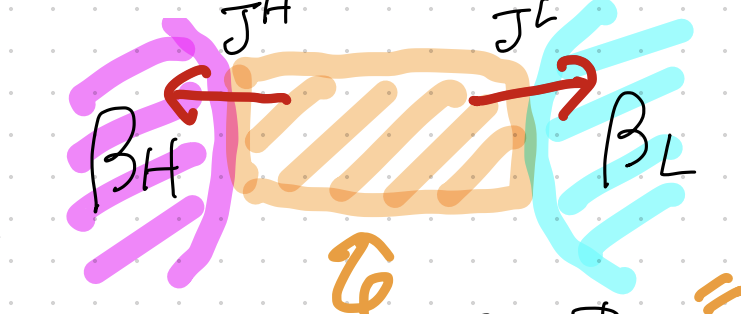
\includegraphics[width=100mm]{set.png}
    \end{center}
    \caption{設定}
    \label{fig:set}
\end{figure}

系が二つの熱浴に接触しているとする。$\alpha = \text{H,L}$で、それぞれの熱浴の逆温度を$\beta_{\alpha}$、遷移レートを$\omega_{j \to k}(t)$、系のエネルギーを$E_j(t)$とする。このとき、局所詳細釣り合い条件は、
\begin{align}
  \log \frac{\omega_{j \to k}(t)}{\omega_{k \to j}(t)} = \beta_{\alpha(j,k)}(E_j(t) - E_k(t))
\end{align}
である。($\alpha(j,k) = \text{H,L}$)\\
熱浴への熱の流れは、
\begin{align}
  {J}^{\alpha}_{j\to k}(t) =
  \begin{cases}
    E_j(t) - E_k(t) & \alpha(j,k) = \alpha\\
    0 & \text{otherwise}
    \end{cases}
\end{align}
である。また、エントロピー生成は、
\begin{align}
  \theta_{j \to k}(t) & \beta_{\alpha(j,k)}(E_j(t) - E_k(t))\\
    &= \beta_{\text{H}}J^{\text{H}}_{j\to k}(t) + \beta_{\text{L}}J^{\text{L}}_{j\to k}(t)
\end{align}
である。\\
\textbf{仮定}\\
\begin{figure}[H]
    \begin{center}
    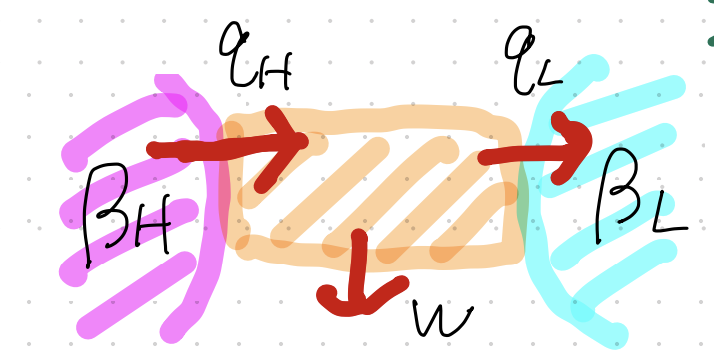
\includegraphics[width=100mm]{set2.png}
    \end{center}
    \caption{仮定}
    \label{fig:set2}
\end{figure}

以下の極限が存在し、その極限値が正であるとする:
\begin{align}
  q_H &= -\lim_{\tau \to \infty}\frac{1}{\tau}\int_0^{\tau} \dd{t}\ev{\hat{J}^H(t)}_t>0\\
  q_L &= \lim_{\tau \to \infty}\frac{1}{\tau}\int_0^{\tau} \dd{t}\ev{\hat{J}^L(t)}_t>0
\end{align}
これは、高温熱浴から系に入ってくる熱流および、低温熱浴に流れる熱流の時間平均である。また、このとき、平均のパワー(仕事率)は、
\begin{align}
  W = q_H - q_L
\end{align}
であり、効率は、
\begin{align}
  \eta = \frac{W}{q_H} = 1 - \frac{q_L}{q_H}
\end{align}
である。このとき、以下の不等式が成立する。

\begin{itembox}[l]{\textbf{Thm:熱機関の、パワーと効率のトレードオフ}}
    熱機関のパワーと効率は、以下の不等式を満たす:
    \begin{align}
      (q_H + q_L)^2 \leq \overline{\Xi} \beta_L q_H (\eta_{\text{C}} - \eta) 
    \end{align}

\end{itembox}
\textbf{Prf}\\
今、
\begin{align}
    \lim_{\tau \to \infty}\frac{1}{\tau}\int_0^{\tau} \dd{t}\ev{\hat{\theta}_t}_t &= -\beta_H q_H + \beta_L q_L\\
    &= -\beta_H q_H + \beta_L (q_H - W)\\
    &= \beta_L q_H \qty(-\frac{\beta_H}{\beta_L} + 1 - \frac{W}{q_H})\\
      &= \beta_L q_H (\eta_{\text{C}} - \eta) (\geq 0)
  \end{align}
  である。また、
\begin{align}
  g_{j \to k}(t) = \hat{J}_{j \to k}^L(t) - \hat{J}_{j \to k}^H(t)
\end{align}
とする。このとき、Shiraishi-Saito不等式より、
\begin{align}
  \left(\frac{1}{\tau}\int_0^{\tau} \dd{t}\ev{\hat{g}(t)}_t\right)^2 \leq \overline{\Xi} \lim_{\tau \to \infty}\frac{1}{\tau}\int_0^{\tau} \dd{t}\ev{\hat{\theta}_t}_t
\end{align}
である。ここで、
\begin{align}
  \overline{\Xi} = \lim_{\tau \to \infty}\frac{1}{\tau} \dd{t} \frac{1}{2}\sum_{j,k(j \neq k)}^{\Omega} R_{kj}(t)p_j(t) (E_j(t) - E_k(t))^2
\end{align}
である。(これは、どれくらいactiveに熱のやり取りをするかを表している。)このとき、
\begin{align}
  \qty(\frac{1}{\tau}\int_0^{\tau} \dd{t}\ev{\hat{g}(t)}_t)^2 = (q_H + q_L)^2
\end{align}
である。よって、
\begin{align}
  (q_H + q_L)^2 \leq \overline{\Xi} \beta_L q_H (\eta_{\text{C}} - \eta)
\end{align}
である。よって示された。\qedsymbol\\

上で得られた不等式を変形すると、
\begin{align}
  \overline{\Xi} \beta_L(\eta_{\text{C}} - \eta) \geq \frac{(q_H + q_L)^2}{q_H} \geq q_H + q_L
\end{align}
となる。これは、効率がカルノーサイクルに近づくと、$q_H, q_L$が0に近づくことを表している。このもとで、パワーは0に近づくことがわかる。\\
あるいは、以下のようにも変形できる:
\begin{align}
  W &\leq \overline{\Xi} \beta_L\frac{q_H}{(q_H + q_L)^2}(\eta_{\text{C}} - \eta)W\\
  &= \overline{\Xi} \beta_L\frac{q_H}{(q_H + q_L)^2}\eta(\eta_{\text{C}} - \eta)\quad (\because W = q_H \eta)\\
    &\leq \overline{\Xi} \beta_L\eta(\eta_{\text{C}} - \eta)
\end{align}
これは、効率がカルノーサイクルに近づくと、パワーが0に近づくことを直接的に示している。\\

\subsection{熱力学的不確定性関係}

\section{その他}
どこにかけばいいのかわからないものをとりあえずここに書いておく。\\

\subsection{平衡状態への緩和}
\begin{itembox}[l]{\textbf{Thm.平衡状態への緩和}}
  $R$が既約であるとき、マスター方程式
  \begin{align}
    \dot{p}(t) = Rp(t)
  \end{align}
  の解は
  \begin{align}
    \lim_{t \to \infty}p(t) = p^{\text{can},\beta}
  \end{align}
  を満たす。
\end{itembox}
\textbf{Prf.}\\
詳細つり合い条件より、
\begin{align}
  R_{kj}p_j^{\text{can},\beta} = R_{jk}p_k^{\text{can},\beta}
\end{align}
である。ここで、
\begin{align}
  \sum_{k=1}^{\Omega}R_{jk} p_k^{\text{can},\beta} &= R_{jj}p_j^{\text{can},\beta} + \sum_{k \neq j}^{\Omega}R_{jk}p_k^{\text{can},\beta}\\
  &= R_{jj}p_j^{\text{can},\beta} + \sum_{k \neq j}^{\Omega}R_{kj}p_j^{\text{can},\beta}\\
  &= \sum_{k=1}^{\Omega}R_{kj}p_j^{\text{can},\beta}\\
  &= 0
\end{align}
である。よって、カノニカル分布はマスター方程式の特解である。このことと、既約な$R$についての収束定理から、示された。\qed\\
なお、非平衡定常状態についても同様の議論ができるが、その場合は具体的な関数形は与えられない。\\

\section{Langevin系}
Langevin系の取り扱いを見ていく。

\subsection{Wiener過程}

\begin{itembox}[l]{\textbf{Def.Wiener過程}}
  Wiener過程$W(t)$とは、遷移確率が以下で与えられるような確率過程である:
  \begin{align}
    P(\Delta W) = \frac{1}{\sqrt{2\pi \Delta t}}\exp(-\frac{(\Delta W)^2}{2\Delta t})
  \end{align}
  ただし、
  \begin{align}
    \Delta W = W(t + \Delta t) - W(t)
  \end{align}
  である。
\end{itembox}
このとき、Wiener過程は一般に特異点をたくさん含むような、性質のあまりよくない関数となる。
実際、
TODOここに説明を追加する。

Wiener過程によって駆動される、以下の微分方程式を考える。
\begin{align}
  \dd{x} = a(x(t),t)\dd{t} + b((tx,t)\times_{\alpha}\dd{W(t)}
\end{align}
ここで、$a(x(t),t), b(x(t),t)$は適当な関数である。この右辺第二項について、上述した$W(t)$の性質の悪さから、積のルールに気を付ける必要がある。例えば、Riemann積分のときは、$b$について、短冊のどの点を取っても積分値が変わらないが、Wiener積分のときは、そうはいかない。
特に、代表的な積のルールとして、Ito積とStratonovich積がある。\\

\begin{itembox}[l]{\textbf{Def.Ito積/Stratonovich積}}
  Ito積とは、
  \begin{align}
   \dd{x}_{\text{I}} = a(x(t),t) \dd{t} + b(x(t),t) \cdot \dd{W(t)} := a(x(t),t) \dd{t} + b(x(t),t)\dd{W(t)}
  \end{align}
  である。また、Stratonovich積とは、
  \begin{align}
    \dd{x}_{\text{S}} = a(x(t),t)\dd{t} + b(x(t),t) \circ \dd{W(t)} := \frac{1}{2}\qty(b(x(t),t) + b(x(t+\dd{t}),t + \dd{t}))\dd{W(t)}
  \end{align}
  である。
\end{itembox}

いかに見るように、これらは互いに相互変換できる。
\begin{itembox}[l]{\textbf{Prop.Ito積とStratonovich積の関係}}
  Ito積とStratonovich積の関係は、
  \begin{align}
    \dd{x}_{\text{S}} = \dd{x}_{\text{I}} + \frac{1}{2}b(x(t),t)\pdv{b(x(t),t)}{x}\dd{t}
  \end{align}
  である。
\end{itembox}
\textbf{Prf.}\\
\begin{align}
  \dd{x}_{\text{S}} &= a(x(t),t)\dd{t} + b(x(t),t) \circ \dd{W(t)}\\
  &= a(x(t),t)\dd{t} + \frac{1}{2}\qty(b(x(t),t) + b(x(t+\dd{t}),t + \dd{t}))\dd{W(t)}\\
  &= a(x(t),t)\dd{t} + b(x(t),t)\dd{W(t)} + \frac{1}{2}\qty(b(x(t+\dd{t}),t + \dd{t}) - b(x(t),t))\dd{W(t)}\\  
  &= a(x(t),t)\dd{t} + b(x(t),t)\dd{W(t)} + \frac{1}{2}\pdv{b(x(t),t)}{x}\dd{x}\dd{W(t)}\quad (\because \dd{W(t)}\dd{t} = 0)\\
  &= \dd{x}_{\text{I}} + \frac{1}{2}b(x(t),t)\pdv{b(x(t),t)}{x}\dd{t} \quad (\because \dd{x} = a(x(t),t)\dd{t} + b(x(t),t)\times_{\alpha} \dd{W(t)})
\end{align}
である。\qed\\

Ito積の性質を調べると、以下のことがわかる。
\begin{itembox}[l]{\textbf{Prop:Ito rule}}
  \begin{align}
    \lim_{N \to \infty}\sum_{i=0}^{N-1}g(x_i,t_i)(\Delta W_i)^2 = \int_0^\tau \dd{t}g(x,t)
  \end{align}
  \begin{align}
    \lim_{N \to \infty}\sum_{i=0}^{N-1}g(x_i,t_i)(\Delta W_i)^n = 0 \quad (n \geq 3)
  \end{align}
  が確率1で成立する。すなわち、
  \begin{align}
    \dd{W^n} &= \delta_{n,2} \dd{t}\\
    \dd{W(t)}\dd{t} &= 0
  \end{align}
  が確率1で成立する。
\end{itembox}
\textbf{Prf.}\\
($n=2$の場合)\\
示すべきことは、
\begin{align}
  \lim_{N \to \infty}\sum_{i=0}^{N-1}g(x_i,t_i)((\Delta W_i)^2 - \Delta t) = 0
\end{align}
が確率1で成り立つことを示すことである。すなわち、左辺の期待値と分散がそれぞれ0になればよい。期待値について、
\begin{align}
  \ev{\sum_{i=0}^{N-1}g(x_i,t_i)((\Delta W_i)^2 - \Delta t)} &= \sum_{i=0}^{N-1}\ev{g(x_i,t_i)}\ev{(\Delta W_i)^2 - \Delta t} \\
  &= 0 \quad (\because \ev{(\Delta W_i)^2 }= \Delta t)
\end{align}
である。分散について、結局$((\Delta W_i)^2-\Delta t)^2$の期待値を計算すればよく、これは、
\begin{align}
  \ev{((\Delta W_i)^2-\Delta t)^2} &= \ev{(\Delta W_i)^4} - 2\Delta t\ev{(\Delta W_i)^2} + \Delta t^2\\
  &= 3\Delta t^2 - 2\Delta t^2 + \Delta t^2\\
  &=2\Delta t^2
\end{align}
である。二乗のオーダーは無視することで、確率1で示された。\footnote{$N \to \infty$とするのでok}\\
($n \geq 3$の場合)\\
上と同様である。\qed\\

\begin{itembox}[l]{\textbf{Thm.Fokker-Planck方程式}}
  Ito型のLangevin方程式
  \begin{align}
    \dd{x}_{\text{I}} = a(x(t),t)\dd{t} + b(x(t),t)\dd{W(t)}
  \end{align}
  に対して、確率密度関数$P(x,t)$は、
  \begin{align}
    \pdv{P(x,t)}{t} = -\pdv{}{x}\qty(a(x,t)P(x,t)) + \frac{1}{2}\pdv[2]{}{x}\qty(b(x,t)^2P(x,t))
  \end{align}
  のように時間発展する。この方程式をFokker-Planck方程式(Ito型)という。\\
  また、Stratonovich型のLangevin方程式
  \begin{align}
    \dd{x}_{\text{S}} = a(x(t),t)\dd{t} + b(x(t),t)\circ \dd{W(t)}
  \end{align}
  に対して、確率密度関数$P(x,t)$は、
  \begin{align}
    \pdv{P(x,t)}{t} = -\pdv{}{x}\qty(a(x,t)P(x,t)) + \frac{1}{2}\pdv{}{x}\qty(b(x,t)\pdv{}{x}\qty(b(x,t)P(x,t)))
  \end{align}
  のように時間発展する。この方程式をFokker-Planck方程式(Stratonovich型)という。
\end{itembox}
\textbf{Prf.}\\
Ito型について証明したのち、変換則に従ってStratonovich型についても示す。\\



\end{document}